% Chapter 8: Seminar - Modern Extensions
% ARFIMA, Machine Learning, LSTM
% Bachelor program, Bucharest University of Economic Studies

\documentclass[9pt, aspectratio=169, t]{beamer}

% Ensure content fits on slides
\setbeamersize{text margin left=8mm, text margin right=8mm}

%=============================================================================
% THEME AND STYLE CONFIGURATION
%=============================================================================
\usetheme{default}
% Using default theme for clean header/footer control

% Color Palette (matching Redispatch PDF)
\definecolor{MainBlue}{RGB}{26, 58, 110}
\definecolor{AccentBlue}{RGB}{26, 58, 110}
\definecolor{IDAred}{RGB}{205, 0, 0}
\definecolor{DarkGray}{RGB}{51, 51, 51}
\definecolor{MediumGray}{RGB}{128, 128, 128}
\definecolor{LightGray}{RGB}{248, 248, 248}
\definecolor{VeryLightGray}{RGB}{235, 235, 235}
\definecolor{KeynoteGray}{RGB}{218, 218, 218}
\definecolor{SectionGray}{RGB}{120, 120, 120}
\definecolor{FooterGray}{RGB}{100, 100, 100}
\definecolor{Crimson}{RGB}{220, 53, 69}
\definecolor{Forest}{RGB}{46, 125, 50}
\definecolor{Amber}{RGB}{181, 133, 63}
\definecolor{Orange}{RGB}{230, 126, 34}
\definecolor{Purple}{RGB}{142, 68, 173}

% Gradient background (exact Keynote 315° gradient: white to RGB 218,218,218)
\setbeamertemplate{background}{%
    \begin{tikzpicture}[remember picture, overlay]
        \shade[shading=axis, shading angle=315,
        top color=white, bottom color=KeynoteGray]
        (current page.south west) rectangle (current page.north east);
    \end{tikzpicture}%
}
% Fallback solid color for compatibility
\setbeamercolor{background canvas}{bg=}

\setbeamercolor{palette primary}{bg=MainBlue, fg=white}
\setbeamercolor{palette secondary}{bg=MainBlue!85, fg=white}
\setbeamercolor{palette tertiary}{bg=MainBlue!70, fg=white}
\setbeamercolor{structure}{fg=MainBlue}
\setbeamercolor{title}{fg=IDAred}
\setbeamercolor{frametitle}{fg=IDAred, bg=}
\setbeamercolor{block title}{bg=MainBlue, fg=white}
\setbeamercolor{block body}{bg=VeryLightGray, fg=DarkGray}
\setbeamercolor{block title alerted}{bg=Crimson, fg=white}
\setbeamercolor{block body alerted}{bg=Crimson!8, fg=DarkGray}
\setbeamercolor{block title example}{bg=Forest, fg=white}
\setbeamercolor{block body example}{bg=Forest!8, fg=DarkGray}
\setbeamercolor{item}{fg=MainBlue}

% Footer colors (override Madrid theme blue)
\setbeamercolor{author in head/foot}{fg=FooterGray, bg=}
\setbeamercolor{title in head/foot}{fg=FooterGray, bg=}
\setbeamercolor{date in head/foot}{fg=FooterGray, bg=}
\setbeamercolor{section in head/foot}{fg=FooterGray, bg=}
\setbeamercolor{subsection in head/foot}{fg=FooterGray, bg=}

% Bullet styles (apply everywhere including blocks)
\setbeamertemplate{itemize item}{\color{MainBlue}$\boxdot$}
\setbeamertemplate{itemize subitem}{\color{MainBlue}$\blacktriangleright$}
\setbeamertemplate{itemize subsubitem}{\color{MainBlue}\tiny$\bullet$}
\setbeamertemplate{itemize/enumerate body begin}{\normalsize}
\setbeamertemplate{itemize/enumerate subbody begin}{\normalsize}

% Item spacing - compact style
\setlength{\leftmargini}{10pt}       % Level 1: minimal indent
\setlength{\leftmarginii}{10pt}      % Level 2: minimal additional indent
% Compact list spacing (zero extra space before/after lists in blocks)
\makeatletter
\def\@listi{\leftmargin\leftmargini \topsep 0pt \parsep 0pt \itemsep 0pt}
\def\@listii{\leftmargin\leftmarginii \topsep 0pt \parsep 0pt \itemsep 0pt}
\makeatother

\setbeamertemplate{navigation symbols}{}

%=============================================================================
% CUSTOM HEADLINE
%=============================================================================
\setbeamertemplate{headline}{%
    \vskip10pt%
    \hbox to \paperwidth{%
        \hskip0.5cm%
        {\small\color{FooterGray}\renewcommand{\hyperlink}[2]{##2}\insertsectionhead}%
        \hfill%
        \textcolor{FooterGray}{\small\insertframenumber}%
        \hskip0.5cm%
    }%
    \vskip4pt%
    {\color{FooterGray}\hrule height 0.4pt}%
}

%=============================================================================
% CUSTOM FOOTER
%=============================================================================
\usepackage{fontawesome5}

\setbeamertemplate{footline}{%
    {\color{FooterGray}\hrule height 0.4pt}%
    \vskip4pt%
    \hbox to \paperwidth{%
        \hskip0.5cm%
        \textcolor{FooterGray}{\small Time Series Analysis and Forecasting}%
        \hfill%
        \raisebox{-0.1em}{%
            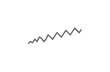
\begin{tikzpicture}[x=0.08em, y=0.08em, line width=0.4pt]
                \draw[FooterGray] (0,3) -- (1,4) -- (2,3.5) -- (3,5) -- (4,4) -- (5,6) -- (6,5.5) -- (7,4) -- (8,5) -- (9,7) -- (10,6) -- (11,5) -- (12,6.5) -- (13,8) -- (14,7) -- (15,6) -- (16,7.5) -- (17,9) -- (18,8) -- (19,7) -- (20,8.5) -- (21,10) -- (22,9) -- (23,8) -- (24,9.5);
            \end{tikzpicture}%
        }%
        \hskip0.5cm%
    }%
    \vskip6pt%
}

%=============================================================================
% PACKAGES
%=============================================================================
\usepackage[utf8]{inputenc}
\usepackage[T1]{fontenc}
\usepackage[english]{babel}
\usepackage{amsmath, amssymb, amsthm}
\usepackage{mathtools}
\usepackage{bm}
\usepackage{tikz}
\usetikzlibrary{arrows.meta, positioning, shapes, calc, decorations.pathreplacing, shadings}
\usepackage{booktabs}
\usepackage{multirow}
\usepackage{array}
\usepackage{graphicx}
\usepackage{hyperref}
\usepackage{colortbl}
\hypersetup{colorlinks=true, linkcolor=MainBlue, urlcolor=MainBlue}
\graphicspath{{../../logos/}{../../charts/}}
\hfuzz=2pt  % Suppress tiny overfull warnings (<2pt)
\vfuzz=2pt  % Suppress tiny vertical overfull warnings (<2pt)

%=============================================================================
% QUANTLET COMMAND
%=============================================================================
\newcommand{\quantlet}[2]{%
    \hfill\href{#2}{%
        \raisebox{-0.15em}{\includegraphics[height=0.7em]{ql_logo.png}}%
        \textcolor{MainBlue}{\tiny\ #1}%
    }%
}

%=============================================================================
% CUSTOM COMMANDS
%=============================================================================
\newcommand{\E}{\mathbb{E}}
\newcommand{\Var}{\text{Var}}
\newcommand{\Cov}{\text{Cov}}

%=============================================================================
% TITLE INFORMATION
%=============================================================================
\title[Chapter 8: Seminar]{Chapter 8: Seminar --- Modern Extensions}
\subtitle{Bachelor program Faculty of Cybernetics, Statistics and Economic Informatics, Bucharest University of Economic Studies, Romania}
\author[Prof. dr. Daniel Traian Pele]{Prof. dr. Daniel Traian Pele\\[0.2cm]\footnotesize\texttt{danpele@ase.ro}}
\institute{Bucharest University of Economic Studies}
\date{Academic Year 2025--2026}

\begin{document}

%=============================================================================
% TITLE SLIDE
%=============================================================================
\begin{frame}[plain]
    \begin{tikzpicture}[remember picture, overlay]
        \fill[IDAred] (current page.north west) rectangle ([yshift=-0.15cm]current page.north east);
        \node[anchor=north west] at ([xshift=0.5cm, yshift=-0.3cm]current page.north west) {
            \href{https://www.ase.ro}{\includegraphics[height=1.1cm]{ase_logo.png}}
        };
        \node[anchor=north] at ([yshift=-0.3cm]current page.north) {
            \href{https://ai4efin.ase.ro}{\includegraphics[height=1.1cm]{ai4efin_logo.png}}
        };
        \node[anchor=north east] at ([xshift=-0.5cm, yshift=-0.3cm]current page.north east) {
            \href{https://www.digital-finance-msca.com}{\includegraphics[height=1.1cm]{msca_logo.png}}
        };
    \end{tikzpicture}
    \vfill
    \begin{center}
        {\Large\textcolor{MediumGray}{Time Series Analysis and Forecasting}}\\[0.3cm]
        {\Huge\textbf{\textcolor{MainBlue}{Chapter 8: Modern Extensions}}}\\[0.5cm]
        {\Large\textcolor{IDAred}{Seminar}}
    \end{center}
    \vfill

    \begin{tikzpicture}[remember picture, overlay]
        \fill[IDAred] (current page.south west) rectangle ([yshift=0.15cm]current page.south east);
        \node[anchor=south west] at ([xshift=0.5cm, yshift=0.8cm]current page.south west) {
            \href{https://theida.net}{\includegraphics[height=0.9cm]{ida_logo.png}}
        };
        \node[anchor=south] at ([xshift=-3cm, yshift=0.8cm]current page.south) {
            \href{https://blockchain-research-center.com}{\includegraphics[height=0.9cm]{brc_logo.png}}
        };
        \node[anchor=south] at ([yshift=0.8cm]current page.south) {
            \href{https://quantinar.com}{\includegraphics[height=0.9cm]{qr_logo.png}}
        };
        \node[anchor=south] at ([xshift=3cm, yshift=0.8cm]current page.south) {
            \href{https://quantlet.com}{\includegraphics[height=0.9cm]{ql_logo.png}}
        };
        \node[anchor=south east] at ([xshift=-0.5cm, yshift=0.8cm]current page.south east) {
            \href{https://ipe.ro/new}{\includegraphics[height=0.9cm]{acad_logo.png}}
        };
    \end{tikzpicture}
\end{frame}

%=============================================================================
% OUTLINE
%=============================================================================
\begin{frame}{Seminar Outline}
    \tableofcontents
\end{frame}

%=============================================================================
% SECTION 1: ARFIMA QUIZ
%=============================================================================
\section{Quiz: ARFIMA and Long Memory}

\begin{frame}{Quiz 1: Hurst Exponent}
    \begin{alertblock}{Question}
        A time series has Hurst exponent $H = 0.8$. What does this indicate?
    \end{alertblock}

    \vspace{0.3cm}

    \begin{enumerate}[A)]
        \item The series is a pure random walk
        \item The series has long memory and is persistent (trend-following)
        \item The series is anti-persistent (mean-reverting)
        \item The series is stationary I(0)
    \end{enumerate}

    \vspace{0.5cm}
    \begin{flushright}\textit{Answer on next slide...}\end{flushright}
\end{frame}

\begin{frame}{Quiz 1: Answer}
    \begin{exampleblock}{Answer: B -- Long memory and persistence}
        \begin{center}
            \includegraphics[width=0.80\textwidth, height=0.50\textheight, keepaspectratio]{ch8_quiz3_hurst.pdf}
        \end{center}
        \vspace{-0.3cm}
        {\footnotesize
        \textbf{Hurst Exponent}: $H = 0.5$ (random walk), $0.5 < H < 1$ (persistence), $0 < H < 0.5$ (mean reversion)
        }
    \end{exampleblock}
\end{frame}

\begin{frame}{Quiz 2: Fractional Differencing Parameter}
    \begin{alertblock}{Question}
        In the ARFIMA(p, d, q) model, the parameter $d$ can take values:
    \end{alertblock}

    \vspace{0.3cm}

    \begin{enumerate}[A)]
        \item Only integer values (0, 1, 2, ...)
        \item Only $d = 0$ or $d = 1$
        \item Any real value, including fractional
        \item Only negative values
    \end{enumerate}

    \vspace{0.5cm}
    \begin{flushright}\textit{Answer on next slide...}\end{flushright}
\end{frame}

\begin{frame}{Quiz 2: Answer}
    \begin{exampleblock}{Answer: C -- Any real value}
        \begin{center}
            \includegraphics[width=0.75\textwidth, height=0.45\textheight, keepaspectratio]{ch8_quiz2_arfima_d.pdf}
        \end{center}
        \vspace{-0.3cm}
        {\footnotesize
        \textbf{Interpretation}: $d = 0$ (ARMA), $0 < d < 0.5$ (long memory, stationary), $0.5 \leq d < 1$ (non-stationary), $d = 1$ (unit root). Relation to Hurst: $d = H - 0.5$
        }
    \end{exampleblock}
\end{frame}

\begin{frame}{Quiz 3: Long Memory in Financial Series}
    \begin{alertblock}{Question}
        In which financial series is long memory most commonly documented?
    \end{alertblock}

    \vspace{0.3cm}

    \begin{enumerate}[A)]
        \item Stock prices
        \item Daily returns
        \item Volatility (squared returns)
        \item Trading volume
    \end{enumerate}

    \vspace{0.5cm}
    \begin{flushright}\textit{Answer on next slide...}\end{flushright}
\end{frame}

\begin{frame}{Quiz 3: Answer}
    \begin{exampleblock}{Answer: C -- Volatility}
        \begin{center}
            \includegraphics[width=0.80\textwidth, height=0.50\textheight, keepaspectratio]{ch8_quiz1_long_memory.pdf}
        \end{center}
        \vspace{-0.3cm}
        {\footnotesize
        \textbf{Stylized facts}: Returns are memoryless ($H \approx 0.5$), volatility has long memory ($H \approx 0.7-0.9$) due to clustering. Basis for FIGARCH/HAR-RV models.
        }
    \end{exampleblock}
\end{frame}

%=============================================================================
% SECTION 2: MACHINE LEARNING QUIZ
%=============================================================================
\section{Quiz: Machine Learning for Time Series}

\begin{frame}{Quiz 4: Feature Engineering}
    \begin{alertblock}{Question}
        To apply Random Forest to time series, we must create:
    \end{alertblock}

    \vspace{0.3cm}

    \begin{enumerate}[A)]
        \item Dummy variables for each observation
        \item Lag features and rolling statistics
        \item Fourier transforms of the series
        \item Only the first difference of the series
    \end{enumerate}

    \vspace{0.5cm}
    \begin{flushright}\textit{Answer on next slide...}\end{flushright}
\end{frame}

\begin{frame}{Quiz 4: Answer}
    \begin{exampleblock}{Answer: B -- Lag features and rolling statistics}
        \begin{center}
            \includegraphics[width=0.80\textwidth, height=0.48\textheight, keepaspectratio]{ch8_quiz4_rf_features.pdf}
        \end{center}
        \vspace{-0.3cm}
        {\footnotesize
        \textbf{Feature Engineering}: Lag features ($y_{t-1}, \ldots, y_{t-k}$), rolling stats (mean, std), calendar features. Transforms forecasting into supervised regression.
        }
    \end{exampleblock}
\end{frame}

\begin{frame}{Quiz 5: Time Series Cross-Validation}
    \begin{alertblock}{Question}
        Why can't we use standard k-fold cross-validation for time series?
    \end{alertblock}

    \vspace{0.3cm}

    \begin{enumerate}[A)]
        \item It's too slow for long series
        \item It violates temporal order and causes data leakage
        \item It only works for classification
        \item It requires too much data
    \end{enumerate}

    \vspace{0.5cm}
    \begin{flushright}\textit{Answer on next slide...}\end{flushright}
\end{frame}

\begin{frame}{Quiz 5: Answer}
    \begin{exampleblock}{Answer: B -- Violates temporal order}
        \begin{center}
            \includegraphics[width=0.80\textwidth, height=0.48\textheight, keepaspectratio]{ch8_quiz5_cv_comparison.pdf}
        \end{center}
        \vspace{-0.3cm}
        {\footnotesize
        \textbf{Problem}: k-fold shuffles randomly, trains on future, tests on past $\Rightarrow$ data leakage. \textbf{Solution}: Time Series Split (Walk-Forward Validation).
        }
    \end{exampleblock}
\end{frame}

\begin{frame}{Quiz 6: Feature Importance in Random Forest}
    \begin{alertblock}{Question}
        Feature importance in Random Forest for time series helps us:
    \end{alertblock}

    \vspace{0.3cm}

    \begin{enumerate}[A)]
        \item Eliminate all low-importance variables
        \item Identify which lags and features are most predictive
        \item Determine Granger causality
        \item Calculate confidence intervals
    \end{enumerate}

    \vspace{0.5cm}
    \begin{flushright}\textit{Answer on next slide...}\end{flushright}
\end{frame}

\begin{frame}{Quiz 6: Answer}
    \begin{exampleblock}{Answer: B -- Identifies predictive features}
        \textbf{Uses of feature importance:}
        \begin{itemize}
            \item Understanding temporal structure
            \item Selecting optimal number of lags
            \item Identifying relevant factors
        \end{itemize}

        \vspace{0.3cm}
        \textbf{Caution:}
        \begin{itemize}
            \item Importance does NOT imply causality
            \item Correlated variables may share importance
            \item Use for interpretation, not causal inference
        \end{itemize}
    \end{exampleblock}
\end{frame}

%=============================================================================
% SECTION 3: LSTM QUIZ
%=============================================================================
\section{Quiz: LSTM Networks}

\begin{frame}{Quiz 7: LSTM Advantage}
    \begin{alertblock}{Question}
        What is the main advantage of LSTM over simple RNNs?
    \end{alertblock}

    \vspace{0.3cm}

    \begin{enumerate}[A)]
        \item It's faster to train
        \item It solves the vanishing/exploding gradient problem
        \item It requires less data
        \item It's easier to interpret
    \end{enumerate}

    \vspace{0.5cm}
    \begin{flushright}\textit{Answer on next slide...}\end{flushright}
\end{frame}

\begin{frame}{Quiz 7: Answer}
    \begin{exampleblock}{Answer: B -- Solves the gradient problem}
        \begin{center}
            \includegraphics[width=0.75\textwidth, height=0.45\textheight, keepaspectratio]{ch8_quiz6_lstm_advantage.pdf}
        \end{center}
        \vspace{-0.3cm}
        {\footnotesize
        \textbf{RNN Problem}: Gradients decay exponentially. \textbf{LSTM Solution}: Cell state (highway), forget/input/output gates control information flow.
        }
    \end{exampleblock}
\end{frame}

\begin{frame}{Quiz 8: Data Preparation for LSTM}
    \begin{alertblock}{Question}
        Before training an LSTM, data should be:
    \end{alertblock}

    \vspace{0.3cm}

    \begin{enumerate}[A)]
        \item Log-transformed
        \item Normalized/scaled to [0,1] or [-1,1]
        \item Differenced twice
        \item Converted to integers
    \end{enumerate}

    \vspace{0.5cm}
    \begin{flushright}\textit{Answer on next slide...}\end{flushright}
\end{frame}

\begin{frame}{Quiz 8: Answer}
    \begin{exampleblock}{Answer: B -- Normalized/scaled}
        \begin{center}
            \includegraphics[width=0.75\textwidth, height=0.45\textheight, keepaspectratio]{ch8_quiz8_data_leakage.pdf}
        \end{center}
        \vspace{-0.3cm}
        {\footnotesize
        \textbf{Why?} Activation functions work in limited ranges; faster convergence; numerical stability.
        \textbf{Methods}: Min-Max $\rightarrow$ [0,1] or Standard (mean 0, std 1). Fit on train only!
        }
    \end{exampleblock}
\end{frame}

\begin{frame}{Quiz 9: LSTM Hyperparameters}
    \begin{alertblock}{Question}
        Which is NOT a typical LSTM hyperparameter?
    \end{alertblock}

    \vspace{0.3cm}

    \begin{enumerate}[A)]
        \item Number of units (neurons) per layer
        \item Input sequence length
        \item Learning rate
        \item Differencing parameter $d$
    \end{enumerate}

    \vspace{0.5cm}
    \begin{flushright}\textit{Answer on next slide...}\end{flushright}
\end{frame}

\begin{frame}{Quiz 9: Answer}
    \begin{exampleblock}{Answer: D -- The $d$ parameter}
        $d$ is specific to ARFIMA models, not LSTM!

        \vspace{0.3cm}
        \textbf{LSTM Hyperparameters:}
        \begin{itemize}
            \item \textbf{Architecture}: number of layers, units/layer
            \item \textbf{Sequence}: lookback length
            \item \textbf{Training}: learning rate, batch size, epochs
            \item \textbf{Regularization}: dropout, early stopping
        \end{itemize}

        \vspace{0.2cm}
        \textbf{Tuning}: Grid search or Bayesian optimization with time series CV
    \end{exampleblock}
\end{frame}

\begin{frame}{Quiz 10: Model Selection}
    \begin{alertblock}{Question}
        When comparing ARFIMA, Random Forest, and LSTM for forecasting:
    \end{alertblock}

    \vspace{0.3cm}

    \begin{enumerate}[A)]
        \item LSTM always wins because it's deep learning
        \item ARFIMA is always best for financial data
        \item The best model depends on data characteristics and problem requirements
        \item Random Forest can't be used for time series
    \end{enumerate}

    \vspace{0.5cm}
    \begin{flushright}\textit{Answer on next slide...}\end{flushright}
\end{frame}

\begin{frame}{Quiz 10: Answer}
    \begin{exampleblock}{Answer: C -- Depends on data and requirements}
        \begin{center}
            \includegraphics[width=0.80\textwidth, height=0.48\textheight, keepaspectratio]{ch8_quiz7_model_selection.pdf}
        \end{center}
        \vspace{-0.3cm}
        {\footnotesize
        \textbf{Guidelines}: ARFIMA (long memory, interpretability), RF (nonlinear, feature importance), LSTM (long sequences, complex patterns). Always validate with time series CV!
        }
    \end{exampleblock}
\end{frame}

%=============================================================================
% TRUE/FALSE QUESTIONS
%=============================================================================
\section{True/False Questions}

\begin{frame}{True/False Questions}
    Determine if each statement is True or False:

    \vspace{0.3cm}
    \begin{enumerate}
        \item The Hurst exponent $H = 0.5$ indicates long memory.
        \item ARFIMA reduces to ARIMA when $d$ is an integer.
        \item Standard k-fold CV is appropriate for time series data.
        \item LSTM can capture long-range dependencies better than simple RNNs.
        \item Feature importance in Random Forest proves causality.
        \item Normalizing data is optional when training neural networks.
    \end{enumerate}

    \vspace{0.3cm}
    \begin{flushright}\textit{Answers on next slide...}\end{flushright}
\end{frame}

\begin{frame}{True/False: Solutions}
    {\small
    \begin{enumerate}\setlength{\itemsep}{1pt}
        \item The Hurst exponent $H = 0.5$ indicates long memory. \hfill \textcolor{Crimson}{\textbf{FALSE}}

        {\footnotesize \textcolor{MediumGray}{$H = 0.5$ means random walk (no memory). Long memory: $H > 0.5$.}}

        \item ARFIMA reduces to ARIMA when $d$ is an integer. \hfill \textcolor{Forest}{\textbf{TRUE}}

        {\footnotesize \textcolor{MediumGray}{With $d = 0$ or $d = 1$, ARFIMA becomes standard ARMA or ARIMA.}}

        \item Standard k-fold CV is appropriate for time series data. \hfill \textcolor{Crimson}{\textbf{FALSE}}

        {\footnotesize \textcolor{MediumGray}{Use time series split to maintain temporal order and avoid data leakage.}}

        \item LSTM can capture long-range dependencies better than simple RNNs. \hfill \textcolor{Forest}{\textbf{TRUE}}

        {\footnotesize \textcolor{MediumGray}{Cell state and gates allow gradients to flow without vanishing.}}

        \item Feature importance in Random Forest proves causality. \hfill \textcolor{Crimson}{\textbf{FALSE}}

        {\footnotesize \textcolor{MediumGray}{Shows predictive power, not causal relationship.}}

        \item Normalizing data is optional when training neural networks. \hfill \textcolor{Crimson}{\textbf{FALSE}}

        {\footnotesize \textcolor{MediumGray}{Critical for convergence and stability with activation functions.}}
    \end{enumerate}
    }
\end{frame}

%=============================================================================
% SECTION 4: PRACTICAL PROBLEMS
%=============================================================================
\section{Practice Problems}

\begin{frame}{Problem 1: Hurst Exponent Estimation}
    \begin{block}{Exercise}
        Given daily Bitcoin returns, estimate the Hurst exponent using the R/S method and interpret the result.
    \end{block}

    \vspace{0.3cm}
    \textbf{Solution Steps:}
    \begin{enumerate}
        \item Calculate mean over subintervals of different lengths $n$
        \item For each $n$: calculate Range($R$) and Std($S$)
        \item The ratio $R/S$ grows as $n^H$
        \item Fit regression: $\log(R/S) = H \cdot \log(n) + c$
    \end{enumerate}

    \vspace{0.2cm}
    \textbf{Python code}: \texttt{nolds.hurst\_rs(returns)}
\end{frame}

\begin{frame}{Problem 1: Solution and Interpretation}
    \begin{exampleblock}{Typical Bitcoin Results}
        \begin{itemize}
            \item Returns: $H \approx 0.45-0.55$ (approximately random walk)
            \item Volatility (|returns|): $H \approx 0.75-0.85$ (long memory!)
        \end{itemize}
    \end{exampleblock}

    \vspace{0.3cm}
    \textbf{Interpretation:}
    \begin{itemize}
        \item Returns are hard to predict (EMH approximately valid)
        \item Volatility is predictable over long horizons
        \item Implications for risk management and VaR
    \end{itemize}

    \vspace{0.2cm}
    \textbf{Application}: FIGARCH models may outperform standard GARCH
\end{frame}

\begin{frame}{Problem 2: Random Forest for Forecasting}
    \begin{block}{Exercise}
        Build a Random Forest model for 1-day ahead Bitcoin price forecasting. Evaluate using TimeSeriesSplit.
    \end{block}

    \vspace{0.3cm}
    \textbf{Pipeline:}
    \begin{enumerate}
        \item \textbf{Feature engineering}:
            \begin{itemize}
                \item Lags: $y_{t-1}, y_{t-2}, \ldots, y_{t-7}$
                \item Rolling mean/std: 7, 14, 30 days
            \end{itemize}
        \item \textbf{Train/Test split}: TimeSeriesSplit(n\_splits=5)
        \item \textbf{Model}: RandomForestRegressor(n\_estimators=100)
        \item \textbf{Evaluation}: RMSE, MAE, Direction Accuracy
    \end{enumerate}
\end{frame}

\begin{frame}{Problem 2: Code and Results}
    \begin{exampleblock}{Python Code}
        {\footnotesize
        \texttt{from sklearn.ensemble import RandomForestRegressor}\\
        \texttt{from sklearn.model\_selection import TimeSeriesSplit}\\[0.2cm]
        \texttt{tscv = TimeSeriesSplit(n\_splits=5)}\\
        \texttt{rf = RandomForestRegressor(n\_estimators=100)}\\[0.2cm]
        \texttt{for train\_idx, test\_idx in tscv.split(X):}\\
        \texttt{~~~~rf.fit(X[train\_idx], y[train\_idx])}\\
        \texttt{~~~~pred = rf.predict(X[test\_idx])}
        }
    \end{exampleblock}

    \vspace{0.2cm}
    \textbf{Typical results}:
    \begin{itemize}
        \item Direction accuracy: 52-55\% (slightly above random)
        \item Feature importance: lag-1 and rolling\_std dominate
    \end{itemize}
\end{frame}

\begin{frame}{Problem 3: LSTM for Time Series}
    \begin{block}{Exercise}
        Implement a simple LSTM model for Bitcoin forecasting. Compare with Random Forest.
    \end{block}

    \vspace{0.3cm}
    \textbf{Simple LSTM Architecture:}
    \begin{enumerate}
        \item Input: 30-day sequences
        \item LSTM layer: 50 units
        \item Dense output: 1 neuron (forecast)
        \item Loss: MSE, Optimizer: Adam
    \end{enumerate}

    \vspace{0.2cm}
    \textbf{Important steps}:
    \begin{itemize}
        \item MinMaxScaler normalization
        \item Reshape to [samples, timesteps, features]
        \item Early stopping to prevent overfitting
    \end{itemize}
\end{frame}

\begin{frame}{Problem 3: LSTM Code}
    \begin{exampleblock}{Keras/TensorFlow Code}
        {\footnotesize
        \texttt{from tensorflow.keras.models import Sequential}\\
        \texttt{from tensorflow.keras.layers import LSTM, Dense}\\[0.2cm]
        \texttt{model = Sequential([}\\
        \texttt{~~~~LSTM(50, input\_shape=(30, 1)),}\\
        \texttt{~~~~Dense(1)}\\
        \texttt{])}\\[0.2cm]
        \texttt{model.compile(optimizer='adam', loss='mse')}\\
        \texttt{model.fit(X\_train, y\_train, epochs=50,}\\
        \texttt{~~~~~~~~~~validation\_split=0.1, verbose=0)}
        }
    \end{exampleblock}

    \vspace{0.2cm}
    \textbf{Typical RF vs LSTM comparison}:
    \begin{itemize}
        \item RMSE similar (LSTM slightly better on smooth data)
        \item RF: faster, more interpretable
        \item LSTM: captures complex patterns better
    \end{itemize}
\end{frame}

%=============================================================================
% SECTION 5: SUMMARY
%=============================================================================
\section{Summary}

\begin{frame}{Summary: When to Use Each Method}
    \begin{block}{ARFIMA}
        \begin{itemize}
            \item Series with long memory (volatility, hydrology)
            \item When $0 < d < 0.5$ is theoretically justified
            \item Statistical interpretability is important
        \end{itemize}
    \end{block}

    \begin{block}{Random Forest}
        \begin{itemize}
            \item Nonlinear relationships between features
            \item Feature importance for understanding
            \item Structured data, not too long series
        \end{itemize}
    \end{block}

    \begin{block}{LSTM}
        \begin{itemize}
            \item Long sequences with complex dependencies
            \item Sufficient data for deep learning
            \item Patterns difficult to capture with classical methods
        \end{itemize}
    \end{block}
\end{frame}

\begin{frame}{Key Formulas}
    \begin{block}{ARFIMA and Long Memory}
        \begin{itemize}
            \item Fractional differencing: $(1-L)^d y_t = \varepsilon_t$
            \item Hurst exponent: $d = H - 0.5$
            \item ACF for long memory: $\rho(k) \sim k^{2d-1}$ (slow decay)
        \end{itemize}
    \end{block}

    \begin{block}{Machine Learning}
        \begin{itemize}
            \item Lag feature: $X_t = [y_{t-1}, y_{t-2}, \ldots, y_{t-k}]$
            \item RMSE: $\sqrt{\frac{1}{n}\sum(y_i - \hat{y}_i)^2}$
            \item Direction Accuracy: $\frac{1}{n}\sum \mathbf{1}[\text{sign}(\Delta y) = \text{sign}(\Delta \hat{y})]$
        \end{itemize}
    \end{block}

    \begin{block}{LSTM}
        \begin{itemize}
            \item Forget gate: $f_t = \sigma(W_f \cdot [h_{t-1}, x_t] + b_f)$
            \item Cell update: $C_t = f_t * C_{t-1} + i_t * \tilde{C}_t$
        \end{itemize}
    \end{block}
\end{frame}

%=============================================================================
% THANK YOU SLIDE
%=============================================================================
\begin{frame}[plain]
    \begin{tikzpicture}[remember picture, overlay]
        \fill[IDAred] (current page.north west) rectangle ([yshift=-0.15cm]current page.north east);
    \end{tikzpicture}
    \vfill
    \begin{center}
        {\Huge\textbf{\textcolor{MainBlue}{Thank You!}}}\\[1cm]
        {\Large Questions?}\\[0.5cm]
        {\large\texttt{danpele@ase.ro}}
    \end{center}
    \vfill
    \begin{tikzpicture}[remember picture, overlay]
        \fill[IDAred] (current page.south west) rectangle ([yshift=0.15cm]current page.south east);
    \end{tikzpicture}
\end{frame}

\end{document}
